% !TEX root = Slide.tex

\title{Pelican e perchè generare\\ siti statici}
\subtitle{senza farsi del male}
\author{Matteo Scarpa \\ @fundor333}
\institute{Pycon 9}

\begin{document}
	\frame{\maketitle}
	
	\begin{frame}
	\frametitle{Chi sono}
		\begin{columns}
			\column{0.5\textwidth}
			\begin{itemize}
				\item Informatico e Pythonista
				\item Sostenitore dell'Open Source
				\item Seguo attivamente Python Italia, Gdg Venezia, DataBeers Venezia
				\item @Fundor333
			\end{itemize}
			\column{0.5\textwidth}
			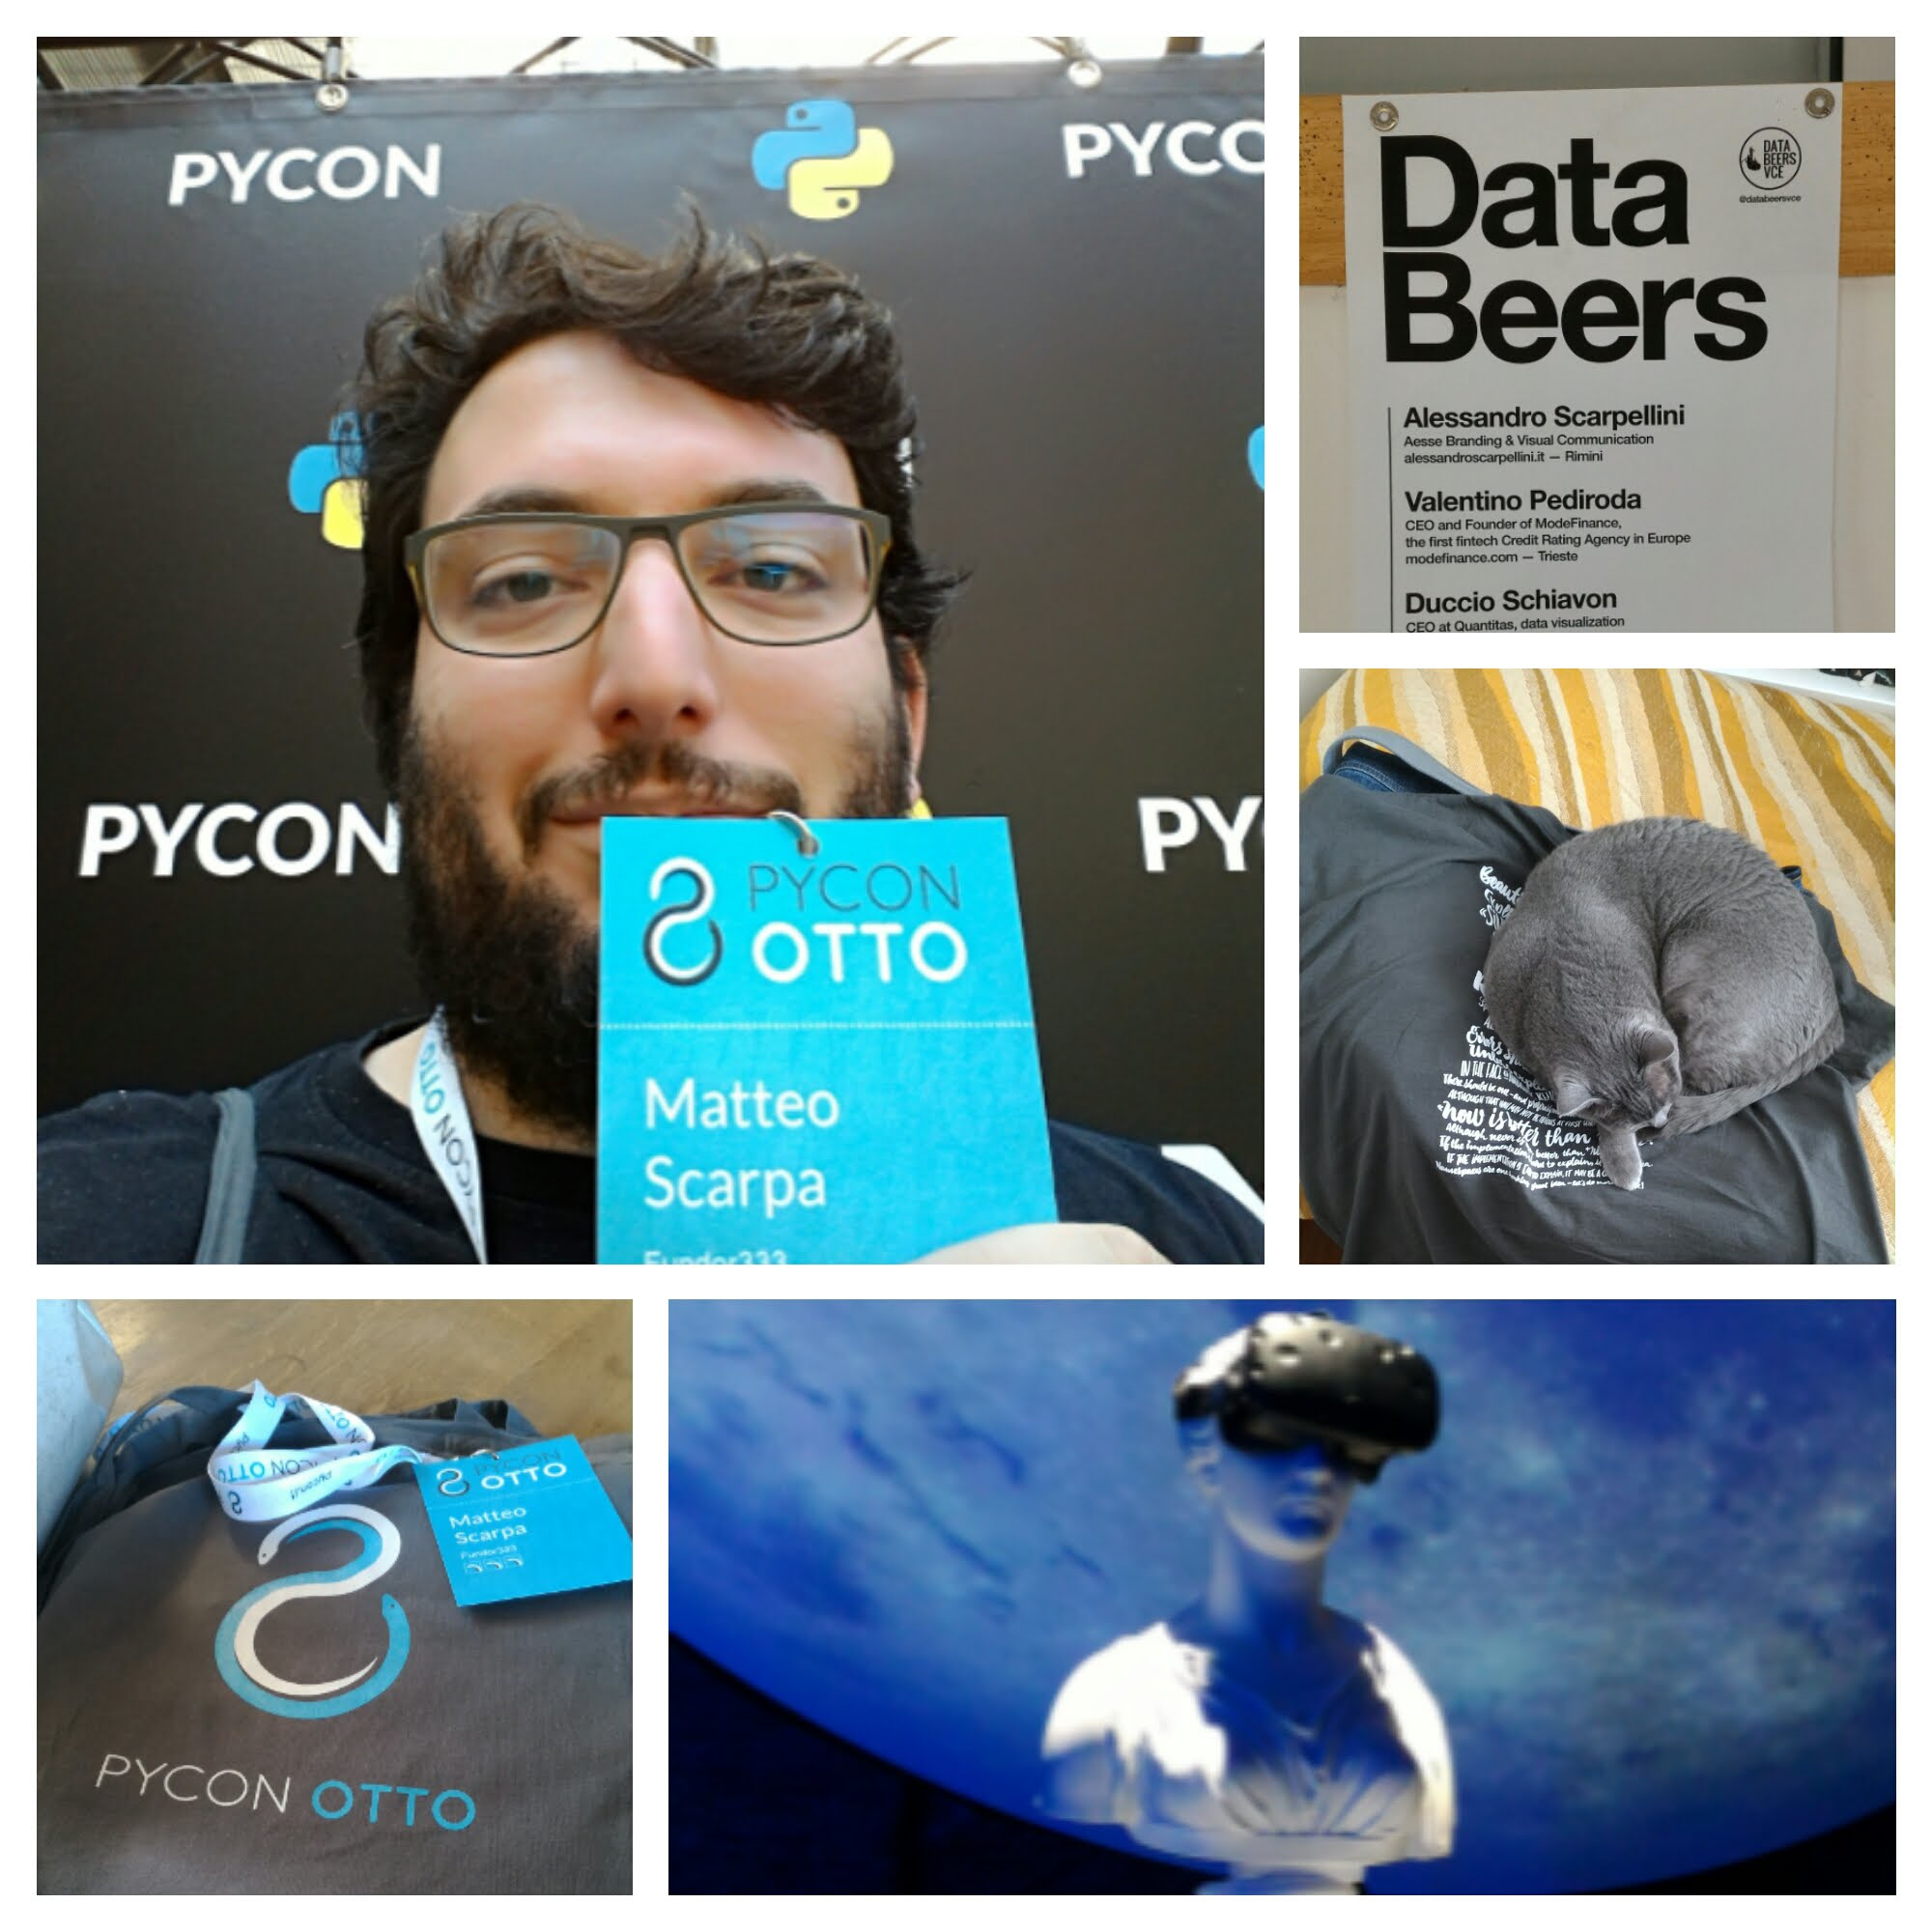
\includegraphics[scale=0.08]{img/foto}
		\end{columns}	
	\end{frame}


	\begin{frame}
		\frametitle{Perchè mi serve un sito?}
	\end{frame}

	\begin{frame}
		\frametitle{Content management system}
	\end{frame}
	
	\begin{frame}
		\frametitle{Static Site Generator}
	\end{frame}

\end{document}
